% =====================================================================
\section{Results}
\label{sec:results}
% =====================================================================
% Every table here is generated from ../results/*.csv by gen_tables.py.
% Unmeasured cells are printed as expected values with a visible note.
% TODO(authors): once the Packet Tracer runs are in, re-read the prose of
% this section against the measured tables and add your interpretation of
% any cell where Packet Tracer differs from the prediction.

\ifmeasured\else
\noindent\fbox{\parbox{\dimexpr\columnwidth-2\fboxsep-2\fboxrule}{\footnotesize\textbf{Data status.} Configuration cost (Tables~\ref{tab:fix} and~\ref{tab:complexity}) is measured. Analyser verdicts are computed from the configurations. Attack, surface, functional and metric values are expected outcomes, marked as such, until the Packet Tracer runs are recorded.}}
\par\medskip
\fi

\subsection{Pre-deployment findings}
\label{sec:res-verify}
\ifhavefix
The analyser and the review found three real defects and one inconsistent expectation before any simulator run (Table~\ref{tab:fix}).

\emph{Router-self-address class (F-1, H-1).} In D2, \cfg{MEDIOT-IN} and \cfg{BLDGIOT-IN} permit IoT traffic to 10.10.20.0/24. That subnet contains the core's own SVI-20 address 10.10.20.1, and the core's VTY lines accept Telnet with a shared password and no \cfg{access-class}. A compromised IoT device could therefore log in to CORE-MLS even though every address the test plan probed was denied, so A4 was partial, not blocked. The review then found the mirror image for guests. \cfg{GUEST-IN} denied only 10.0.0.0/8, but EDGE-RTR's WAN address 198.51.100.2 lies outside that range and has the same weak VTY. A guest could open a session on the edge router, and from there on the core. In both cases the ACL names a range and forgets that a router also owns an address in, or just outside, that range. The fixes are one deny each, placed before the zone permit (Table~\ref{tab:acl}). The analyser confirms that both management paths close, and the IoT node's reach in D2 falls from \fixHostsDtwoPre{}/\fixSvcDtwoPre{} to \fixHostsDtwoPost{}/\fixSvcDtwoPost{} hosts/services. D3 was never affected: host-specific permits exclude every gateway address, and VTY access is limited to VLAN~99.

\emph{UDP/67 exfiltration (F-3).} Every SVI ACL in D2 and D3 began with \cfg{permit udp any any eq 67}, so DHCP could work before a client had an address. That line also lets UDP/67 leave through PAT to any Internet host, a one-way channel that survived micro-segmentation. Restricting it to the broadcast address and the DHCP server closes the channel, and all nine functional tests still pass.

\emph{Unhardened server switch (F-4).} The 21 unused SW-SRV ports in D3 were up in VLAN~1 on the firewall's trusted side, and they are now parked and shut. Finally, the A3 expectation for D2 at L3 was corrected to partial. The cross-class target Pump-A1 sits in another VLAN, so \cfg{BLDGIOT-IN} denies it (F-2).

The fixes add \fixDeltaDtwo{} lines (\fixDeltaAcesDtwo{} ACEs) to D2 and \fixDeltaDthree{} (\fixDeltaAcesDthree{}) to D3. With them, the analyser's verdicts disagree with the expected matrix in \fixDisDtwoPost{} of the 15 D2 attack runs, against \fixDisDtwoPre{} before.
\fi

% AUTO-GENERATED by paper/gen_tables.py -- do not edit by hand; edit the data and re-run.
\begin{table}[t]
\centering
\caption{Pre-deployment fixes (F-1, H-1, F-3, F-4) recomputed by the static analyser on the archived pre-fix and the current configurations. Lines and ACEs are counted; the other columns are analyser predictions. A4: verdict at L1/L2/L3; H/S: hosts/services reachable from the IoT node; G$\rightarrow$E: guest can open a management session on EDGE-RTR's WAN address; U67: UDP/67 reaches the Internet; Idle: unused SW-SRV ports left up (F-4 concerns D3 only).}
\label{tab:fix}
\scriptsize
\setlength{\tabcolsep}{3pt}
\begin{tabular}{@{}lccccccc@{}}
\toprule
 & Lines & ACEs & A4 & H/S & G$\rightarrow$E & U67 & Idle \\
\midrule
D2 pre-fix & 293 & 11 & P/P/P & 9/5 & yes & yes & 21 \\
D2 post-fix & 302 & 17 & B/B/B & 8/4 & no & no & 21 \\
\midrule
D3 pre-fix & 559 & 47 & B/B/B & 2.7/1 & no & yes & 21 \\
D3 post-fix & 571 & 52 & B/B/B & 2.7/1 & no & no & 0 \\
\bottomrule
\end{tabular}
\end{table}


\subsection{Functional preservation (RQ2)}
All nine legitimate flows pass in every design (Table~\ref{tab:functional})\expnote; the analyser predicts the same. Each D3 permit was written for one of these flows. F3 and F8 use TCP~80 to 10.10.20.12. F4 uses the DHCP permits. F9 uses the four ASA entries that admit Syslog and NTP only from the two transit /30s. F7 moves from Telnet to SSH but stays available from VLAN~99.

% AUTO-GENERATED by paper/gen_tables.py -- do not edit by hand; edit the data and re-run.
\begin{table}[t]
\centering
\caption{Functional preservation: legitimate flows that must keep working in every design (\cmark~pass, \xmark~fail). \textit{(expected, not yet measured)}}
\label{tab:functional}
\footnotesize
\setlength{\tabcolsep}{4pt}
\begin{tabular}{@{}llcccc@{}}
\toprule
ID & Legitimate flow & D0 & D1 & D2 & D3 \\
\midrule
F1 & Staff PC opens EHR by name (DNS+HTTP) & \cmark & \cmark & \cmark & \cmark \\
F2 & Staff PC pings EHR-SRV & \cmark & \cmark & \cmark & \cmark \\
F3 & All 8 IoT devices on IOT-REG-SRV & \cmark & \cmark & \cmark & \cmark \\
F4 & DHCP lease in the correct subnet & \cmark & \cmark & \cmark & \cmark \\
F5 & Guest phone reaches Internet web & \cmark & \cmark & \cmark & \cmark \\
F6 & Staff Internet access via PAT & \cmark & \cmark & \cmark & \cmark \\
F7 & NetAdmin manages switches (Telnet/SSH) & \cmark & \cmark & \cmark & \cmark \\
F8 & IoT rule: smoke $\rightarrow$ HVAC fan & \cmark & \cmark & \cmark & \cmark \\
F9 & Syslog server receives device logs & \cmark & \cmark & \cmark & \cmark \\
\midrule
\multicolumn{2}{@{}l}{Pass rate} & 9/9 & 9/9 & 9/9 & 9/9 \\
\bottomrule
\end{tabular}
\end{table}


\subsection{Attack outcomes}
Table~\ref{tab:attacks} gives the outcome matrix\expnote. D1 blocks nothing (\succeededDone{} of \nAttacks{} succeed), because CORE-MLS routes between all SVIs. This reproduces the finding of Sifawa et al.~\cite{Sifawa2026ImplementationEvaluation} with an IoMT attacker. D2 blocks infrastructure access (A4, after F-1) and the guest pivot (A7). It does not protect the EHR (A2): \cfg{permit ip} admits the whole server subnet on every port. A5 and A6 are Layer-2 attacks inside one VLAN, which no SVI ACL sees. D3 blocks \blockedDthree{} of \nAttacks{}. \cfg{MONITORS-IN} has no entry for the EHR, and the ASA admits the EHR only from staff. DHCP snooping drops the rogue server's OFFER on the untrusted Fa0/5, and the sticky MAC on Fa0/2 err-disables the port when the laptop appears. A1 and A3 stay partial by construction. Same-VLAN peers answer at Layer~2 without crossing an SVI, and TCP~80 to the registration server must stay open. The rogue switch (A8) forms a trunk only in D0, whose ports are dynamic; access-mode ports refuse DTP, and in D3 BPDU Guard also err-disables the port. Q1 can act only where an SVI ACL produces deny counters, that is in D2 and D3\ifhaveqone, with a mean time to contain of \qOneContain~s\fi.

% AUTO-GENERATED by paper/gen_tables.py -- do not edit by hand; edit the data and re-run.
\begin{table}[t]
\centering
\caption{Attack outcome per design (majority vote over all locations $\times$ trials; ties go to the worse outcome). \oS{}~succeeded, \oP{}~partial, \oB{}~blocked; for Q1, \oB{} means the node was detected and quarantined. \textit{(expected, not yet measured)}}
\label{tab:attacks}
\footnotesize
\setlength{\tabcolsep}{4pt}
\begin{tabular}{@{}llcccc@{}}
\toprule
ID & Attack & D0 & D1 & D2 & D3 \\
\midrule
A1 & Recon ping sweep & \oS & \oS & \oP & \oP \\
A2 & EHR access (HTTP) & \oS & \oS & \oS & \oB \\
A3 & IoT-server / cross-class & \oS & \oS & \oS & \oP \\
A4 & Telnet/SSH to infra & \oS & \oS & \oB & \oB \\
A5 & Rogue DHCP server & \oS & \oS & \oS & \oB \\
A6 & Unauthorised device & \oS & \oS & \oS & \oB \\
A7 & Guest $\rightarrow$ EHR pivot & \oS & \oS & \oB & \oB \\
\midrule
A8 & Rogue switch (DTP) & \oS & \oB & \oB & \oB \\
Q1 & Auto-quarantine & \oS & \oS & \oB & \oB \\
\bottomrule
\end{tabular}
\end{table}


\subsection{Attack surface and derived metrics (RQ1)}
Reachable hosts fall from \hostsPctDzero\% (D0, D1) to \hostsPctDtwo\% (D2) and \hostsPctDthree\% (D3), and reachable services from \svcPctDzero\% to \svcPctDtwo\% and \svcPctDthree\% (Table~\ref{tab:surface})\expnote. In D2 the reachable hosts are the four servers and four same-VLAN IoT peers. In D3 they are only same-VLAN peers: two monitors from L1 and L2, four building devices from L3. Location matters only in D3, which is the source of its standard deviation; Packet Tracer outcomes do not vary between trials.
\ifhavemetrics
Weighting reachable hosts by criticality makes the step from D2 to D3 larger. $\mathrm{BR}_w$ falls from \brwDzero{} to \brwDtwo{} and \brwDthree{} (Table~\ref{tab:metrics}), because D2 still exposes the EHR and, from the wards, both pumps. Blocked attempts differ significantly between D1 and D2 ($p=\fisherDtwo$) and between D2 and D3 ($p=\fisherDthree$)\expnote.
\fi

% AUTO-GENERATED by paper/gen_tables.py -- do not edit by hand; edit the data and re-run.
\begin{table}[t]
\centering
\caption{Attack surface reachable from the compromised node: hosts answering (of 23) and services accepting a connection (of 10); per-location means and overall mean$\pm$sd over 3 locations $\times$ trials. \textit{(expected, not yet measured)}}
\label{tab:surface}
\scriptsize
\setlength{\tabcolsep}{3pt}
\begin{tabular}{@{}lrrrrrrr@{}}
\toprule
& \multicolumn{5}{c}{Hosts reachable} & \multicolumn{2}{c}{Services} \\
\cmidrule(lr){2-6}\cmidrule(l){7-8}
Design & L1 & L2 & L3 & mean$\pm$sd & \% & mean$\pm$sd & \% \\
\midrule
D0 Flat & 23 & 23 & 23 & 23.00$\pm$0.00 & 100 & 10.00$\pm$0.00 & 100 \\
D1 VLAN-only & 23 & 23 & 23 & 23.00$\pm$0.00 & 100 & 10.00$\pm$0.00 & 100 \\
D2 Zone ACL & 8 & 8 & 8 & 8.00$\pm$0.00 & 35 & 4.00$\pm$0.00 & 40 \\
D3 Micro-seg & 2 & 2 & 4 & 2.67$\pm$1.00 & 12 & 1.00$\pm$0.00 & 10 \\
\bottomrule
\end{tabular}
\par\vspace{2pt}\parbox{\columnwidth}{\scriptsize L1 = L1-WardA-MedIoT; L2 = L2-WardB-MedIoT; L3 = L3-BuildingIoT. sd is the sample standard deviation over all runs of a design, so it mixes location and trial variation.}
\end{table}

\ifhavemetrics% AUTO-GENERATED by paper/gen_tables.py -- do not edit by hand; edit the data and re-run.
\begin{table}[t]
\centering
\caption{Derived security metrics (tools/metrics.py): attack-surface reduction (ASR), criticality-weighted blast radius (BR$_w$), attack block rate (ABR), policy-compliance rate (PCR), detection coverage (DET) and Fisher's exact $p$ for blocked attempts against the previous design. \textit{(expected, not yet measured)}}
\label{tab:metrics}
\footnotesize
\setlength{\tabcolsep}{4pt}
\begin{tabular}{@{}lcccccc@{}}
\toprule
Design & ASR & BR$_w$ & ABR & PCR & DET & $p$ vs prev. \\
\midrule
D0 Flat & 0.00 & 1.00 & 0.00 & 0.17 & -- & -- \\
D1 VLAN-only & 0.00 & 1.00 & 0.00 & 0.17 & -- & 1 \\
D2 Zone ACL & 0.65 & 0.39 & 0.27 & 0.39 & -- & 2.1e-04 \\
D3 Micro-seg & 0.88 & 0.12 & 0.60 & 0.67 & -- & 0.0027 \\
\bottomrule
\end{tabular}
\par\vspace{2pt}\parbox{\columnwidth}{\scriptsize BR$_w$ weights each reachable host by an asset-criticality score (1--5) assigned by the authors (EHR and pumps 5; infrastructure and monitors 4). Packet Tracer outcomes are deterministic, so $p$ reflects the number of attempts, not run-to-run noise.}
\end{table}
\fi

\subsection{Configuration cost and overhead (RQ3)}
Configuration grows from \cfgLinesDzero{} lines in D0 to \cfgLinesDone{}, \cfgLinesDtwo{} and \cfgLinesDthree{} ($\times$\lineRatioDthree{}), and ACEs from \acesDzero{} to \acesDone{}, \acesDtwo{} and \acesDthree{} (Table~\ref{tab:complexity}). The steps are uneven. D0$\rightarrow$D1 costs \deltaLinesDone{} lines and no ACEs, D1$\rightarrow$D2 \deltaLinesDtwo{} lines on one device, and D2$\rightarrow$D3 \deltaLinesDthree{} lines across six existing devices and the new ASA. Of D3's \acesDthree{} ACEs, \aceCoreDthree{} sit on the core SVIs, \aceAsaDthree{} on the ASA and \aceStdDthree{} in the standard VTY and NAT lists. Fig.~\ref{fig:tradeoff} plots attacks blocked against lines. The curve is flat from D0 to D1 and steepest from D1 to D2. On the legitimate path, D3 adds one Layer-3 device (the ASA) and one policy evaluation between staff and the EHR (Appendix Table~\ref{tab:overhead}). \ifhaveoverhead The measured RTT and hop counts are given there. \else The RTT and hop-count test O1 has not yet been run. \fi

% AUTO-GENERATED by paper/gen_tables.py -- do not edit by hand; edit the data and re-run.
\begin{table}[t]
\centering
\caption{Configuration complexity per design, counted from the device configuration files (comments and mode-change wrappers excluded).}
\label{tab:complexity}
\footnotesize
\begin{tabular}{@{}lrrrr@{}}
\toprule
Design & Devices & Config lines & ACEs & Sec.\ features \\
\midrule
D0 Flat & 7 & 189 ($\times$1.00) & 1 & 0 \\
D1 VLAN-only & 7 & 274 ($\times$1.45) & 1 & 1 \\
D2 Zone ACL & 7 & 302 ($\times$1.60) & 17 & 2 \\
D3 Micro-seg & 8 & 571 ($\times$3.02) & 52 & 12 \\
\bottomrule
\end{tabular}
\end{table}


\begin{figure}[t]
\centering
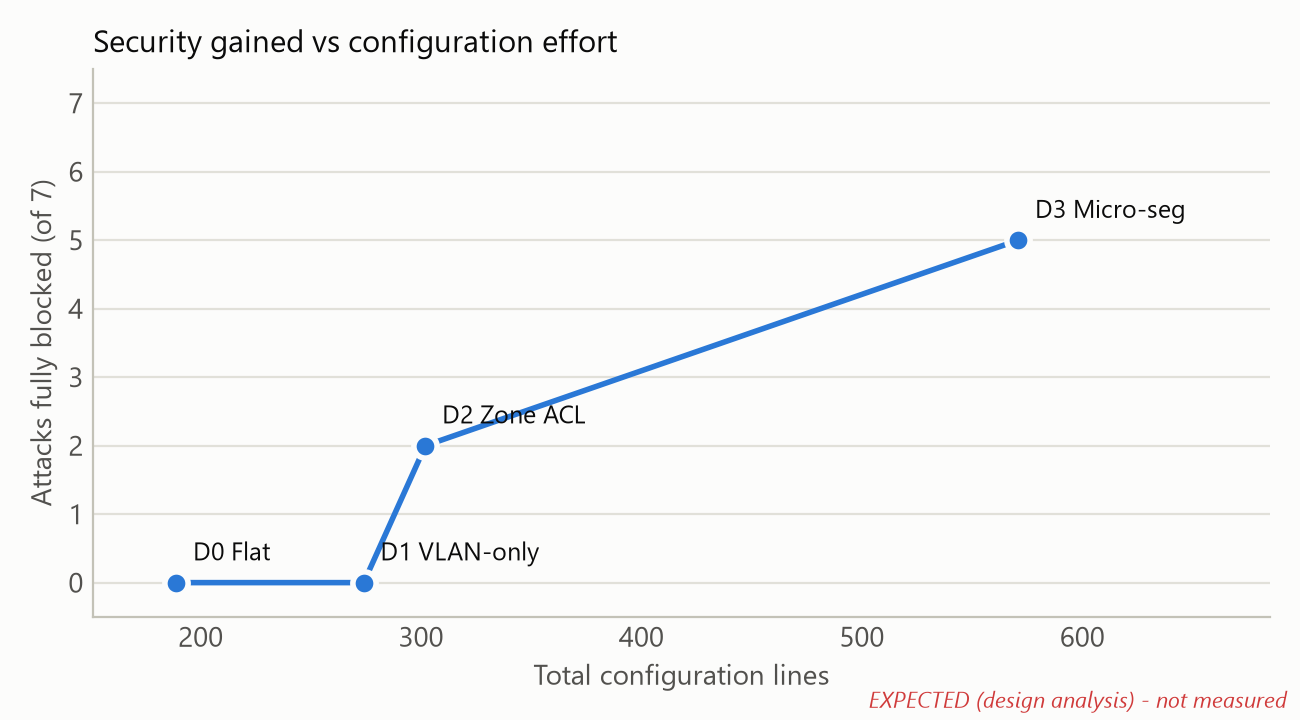
\includegraphics[width=\columnwidth]{tradeoff.png}
\caption{Core attacks fully blocked (of 7) versus total configuration lines per design.\expnote}
\label{fig:tradeoff}
\end{figure}
